\documentclass[tikz,border=5pt]{standalone}

\usepackage{comment}
\usepackage{graphicx}
\usepackage{tikz}
\usetikzlibrary{positioning} % for "below=..." etc.

\usepackage[scaled]{helvet}
\renewcommand{\sfdefault}{phv} % adobe helvetica

\renewcommand{\familydefault}{\sfdefault}

\usepackage[scaled]{helvet}
\renewcommand{\sfdefault}{phv}
\renewcommand{\familydefault}{\sfdefault} % <- add this


\begin{document}
\begin{tikzpicture}[%
  font=\fontfamily{phv}\selectfont,
  every node/.style={inner sep=0, outer sep=0},
  node distance=0.5cm and 0.5cm
]



% === Model 3 row ===
\node[font=\footnotesize\selectfont\fontfamily{phv},anchor=north west, align=center] (m1label) at (-0.6,3.2) {{Model 1}\\ {(p=1)}};
\node[font=\fontsize{7pt}{9pt}\selectfont\fontfamily{phv},anchor=west] (m1truthlabel) at (1, 3.2) {Truth};
\node[right=0.2cm of m1truthlabel.east, anchor=west] (m1truth)
  {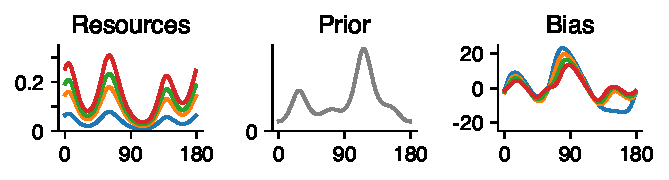
\includegraphics[width=0.42\textwidth]{figures/CounterfactualModel_VIZNoAttRep.py_2345_FOURIER_111_FOURIER_211_1_0_10.0_180.pdf}};
\node[font=\footnotesize\selectfont\fontfamily{phv},left=0.5cm of m1truth, xshift=0.6cm, yshift=0.5cm](label-a){\small a};
\node[font=\fontsize{7pt}{9pt}\selectfont\fontfamily{phv},below=0.9cm of m1truthlabel.south, anchor=north] (m1fittedlabel) {Fitted};
\node[below=0.2cm of m1truth.south, anchor=north] (m1fitted)
  {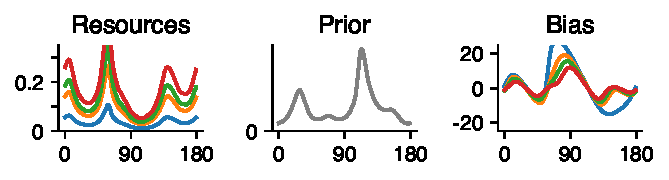
\includegraphics[width=0.42\textwidth]{figures/RunSynthetic_FreePrior_L1Loss_OnSim_VIZNoAttRep.py_SimulateSynthetic_Parameterized_OtherNoiseLevels_Grid_VarySize.py_180_1_2345_N10000_FOURIER_111_FOURIER_211.txt_1_0_10.0_180.pdf}};
\node[below=1cm of label-a](label-b){\small b};
\node[right=1cm of m1truth.east, anchor=center] (temp2){};
\node[font=\fontsize{6pt}{8pt}\selectfont\fontfamily{phv},above=0.1cm of temp2, anchor=center, align=center] (m1nlllabel) {{{negative}}\\ {{log-likelihood}}};
\node[below=0.2cm of m1nlllabel, anchor=north] (m1nll)
  {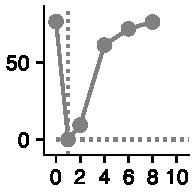
\includegraphics[width=0.12\textwidth]{figures/evaluateCrossValidationResults_Synthetic_Gardelle_Figure4.py_SimulateSynthetic_Parameterized_OtherNoiseLevels_Grid_VarySize.py_180_1_2345_N10000_FOURIER_111_FOURIER_211.txt_RelativeLF.pdf}};
\node[font=\footnotesize\selectfont\fontfamily{phv},left=0.5cm of m1nll, xshift=0.5cm, yshift=1.7cm](label-c){\small c};



% === Model 2 row ===
\node[font=\footnotesize\selectfont\fontfamily{phv},anchor=north west, align=center] (m2label) at (-0.6,-0.2) {{Model 2}\\ {(p=2)}};
\node[font=\fontsize{7pt}{9pt}\selectfont\fontfamily{phv},anchor=west] at (1,0) (m2truthlabel) {Truth};
\node[right=0.2cm of m2truthlabel.east, anchor=west] (m2truth)
  {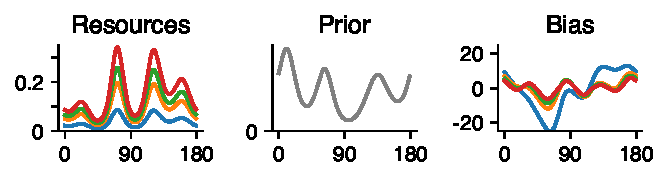
\includegraphics[width=0.42\textwidth]{figures/CounterfactualModel_VIZNoAttRep.py_2345_FOURIER_121_FOURIER_221_2_0_10.0_180.pdf}};
\node[font=\footnotesize\selectfont\fontfamily{phv},left=0.5cm of m2truth, xshift=0.6cm, yshift=0.5cm](label-d){\small d};  
\node[font=\fontsize{7pt}{9pt}\selectfont\fontfamily{phv},below=0.9cm of m2truthlabel.south, anchor=north] (m2fittedlabel) {Fitted};
\node[below=0.2cm of m2truth.south, anchor=north] (m2fitted)
  {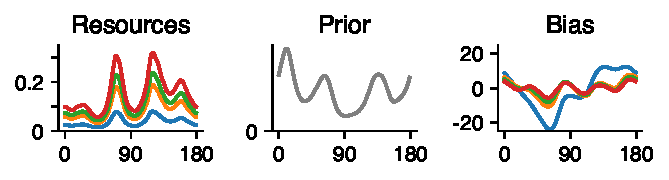
\includegraphics[width=0.42\textwidth]{figures/RunSynthetic_FreePrior_CosineLoss_OnSim_VIZNoAttRep.py_SimulateSynthetic_Parameterized_OtherNoiseLevels_Grid_VarySize.py_180_2_2345_N10000_FOURIER_121_FOURIER_221.txt_2_0_10.0_180.pdf}};
\node[below=1cm of label-d](label-e){\small e};
\node[right=1cm of m2truth.east, anchor=center] (temp0){};
\node[font=\fontsize{6pt}{8pt}\selectfont\fontfamily{phv},above=0.1cm of temp0, anchor=center, align=center] (m2nlllabel) {{{negative}}\\ {{log-likelihood}}};
\node[below=0.2cm of m2nlllabel, anchor=north] (m2nll)
  {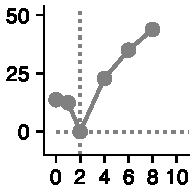
\includegraphics[width=0.12\textwidth]{figures/evaluateCrossValidationResults_Synthetic_Gardelle_Figure4.py_SimulateSynthetic_Parameterized_OtherNoiseLevels_Grid_VarySize.py_180_2_2345_N10000_FOURIER_121_FOURIER_221.txt_RelativeLF.pdf}};
\node[font=\footnotesize\selectfont\fontfamily{phv},left=0.5cm of m2nll, xshift=0.5cm, yshift=1.7cm](label-f){\small f};

% === Model 3 row ===
\node[font=\footnotesize\selectfont\fontfamily{phv},below=6.4cm of m1label.center, anchor=center, align=center] (m3label) {{Model 3}\\ {(p=4)}};
\node[font=\fontsize{7pt}{9pt}\selectfont\fontfamily{phv},below=3.2cm of m2truthlabel.west, anchor=west] (m3truthlabel) {Truth};
\node[right=0.2cm of m3truthlabel.east, anchor=west] (m3truth)
  {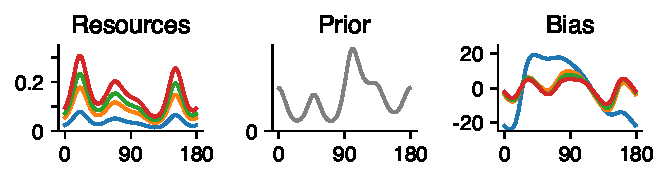
\includegraphics[width=0.42\textwidth]{figures/CounterfactualModel_VIZNoAttRep.py_2345_FOURIER_141_FOURIER_241_4_0_10.0_180.pdf}};
\node[font=\footnotesize\selectfont\fontfamily{phv},left=0.5cm of m3truth, xshift=0.6cm, yshift=0.5cm](label-g){\small g};  
\node[font=\fontsize{7pt}{9pt}\selectfont\fontfamily{phv},below=0.9cm of m3truthlabel.south, anchor=north] (m3fittedlabel) {Fitted};
\node[below=0.2cm of m3truth.south, anchor=north] (m3fitted)
  {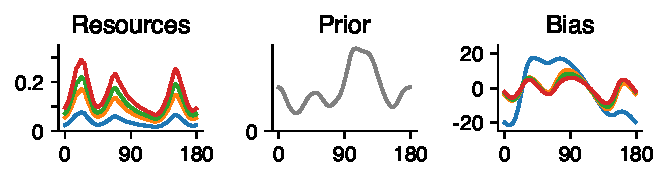
\includegraphics[width=0.42\textwidth]{figures/RunSynthetic_FreePrior_CosineLoss_OnSim_VIZNoAttRep.py_SimulateSynthetic_Parameterized_OtherNoiseLevels_Grid_VarySize.py_180_4_2345_N10000_FOURIER_141_FOURIER_241.txt_4_0_10.0_180.pdf}};
\node[font=\footnotesize\selectfont\fontfamily{phv},below=1cm of label-g](label-h){\small h};
\node[right=1cm of m3truth.east, anchor=center] (temp1){};
\node[font=\fontsize{6pt}{8pt}\selectfont\fontfamily{phv},above=0.1cm of temp1, anchor=center, align=center] (m3nlllabel) {{{negative}}\\ {{log-likelihood}}};
\node[below=0.2cm of m3nlllabel, anchor=north] (m3nll)
  {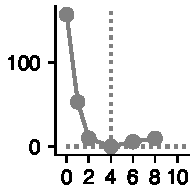
\includegraphics[width=0.12\textwidth]{figures/evaluateCrossValidationResults_Synthetic_Gardelle_Figure4.py_SimulateSynthetic_Parameterized_OtherNoiseLevels_Grid_VarySize.py_180_4_2345_N10000_FOURIER_141_FOURIER_241.txt_RelativeLF.pdf}};
\node[font=\selectfont\fontfamily{phv},left=0.5cm of m3nll, xshift=0.5cm, yshift=1.7cm](label-i){\small i};

\end{tikzpicture}

\begin{comment}

python3 CounterfactualModel_VIZNoAttRep.py 1 0 10.0 180 FOURIER_111 FOURIER_211 2345
python3 CounterfactualModel_VIZNoAttRep.py 2 0 10.0 180 FOURIER_121 FOURIER_221 2345
python3 CounterfactualModel_VIZNoAttRep.py 4 0 10.0 180 FOURIER_141 FOURIER_241 2345
python3 RunSynthetic_FreePrior_L1Loss_OnSim_VIZNoAttRep.py 1 0 10.0 180 SimulateSynthetic_Parameterized_OtherNoiseLevels_Grid_VarySize.py_180_1_2345_N10000_FOURIER_111_FOURIER_211.txt
python3 RunSynthetic_FreePrior_CosineLoss_OnSim_VIZNoAttRep.py 2 0 10.0 180 SimulateSynthetic_Parameterized_OtherNoiseLevels_Grid_VarySize.py_180_2_2345_N10000_FOURIER_121_FOURIER_221.txt
python3 RunSynthetic_FreePrior_CosineLoss_OnSim_VIZNoAttRep.py 4 0 10.0 180 SimulateSynthetic_Parameterized_OtherNoiseLevels_Grid_VarySize.py_180_4_2345_N10000_FOURIER_141_FOURIER_241.txt

python3 evaluateCrossValidationResults_Synthetic_Gardelle_Figure4.py SimulateSynthetic_Parameterized_OtherNoiseLevels_Grid_VarySize.py_180_1_2345_N10000_FOURIER_111_FOURIER_211.txt
python3 evaluateCrossValidationResults_Synthetic_Gardelle_Figure4.py SimulateSynthetic_Parameterized_OtherNoiseLevels_Grid_VarySize.py_180_2_2345_N10000_FOURIER_121_FOURIER_221.txt
python3 evaluateCrossValidationResults_Synthetic_Gardelle_Figure4.py SimulateSynthetic_Parameterized_OtherNoiseLevels_Grid_VarySize.py_180_4_2345_N10000_FOURIER_141_FOURIER_241.txt

#
#To reproduce figure 4 in the main paper, run these three scirpts in order:
#
#1. run\_data\_sampling\_fig4.sh
#
#2. run\_ground\_truth\_fitting\_fig4.sh
#
#3. run\_cross\_fitting\_fig4.sh
#
#If you want to generate new datasets, run `python3 SimulateSynthetic_Parameterized_OtherNoiseLevels_Grid_VarySize.py {GroundTruthExponent} 0 10.0 180 10000 FOURIER_{Paramter1} FOURIER_{Parameter2} {NoiseLevels}`, where exponent = {0|1|2|4|6|8}, parameter1, paramer2 can be two arbitrary numbers.
#
#To visualize the generated datasets, run `python3 CounterfactualModel_VIZ.py {GroundTruthExponent} 0 10.0 180 FOURIER_{Parameter1} FOURIER_{Parameter2}`.
#
#To fit datasets and visualize the fitting result, run `python3 RunSynthetic_FreePrior_{LossType}Loss_OnSim.py {FittingExponent} 0 10.0 180 SimulateSynthetic_Parameterized_OtherNoiseLevels_Grid_VarySize.py_180_{GroundTruthExponent}_{NoiseLevels}_N10000_FOURIER_{Parameter1}_FOURIER_{Parameter2}.txt`, where LossType =
#
#* MAP, FittingExponent = 0
#
#* L1, FittingExponent = 1
#
#* Cosine, FittingExponent > 1
#
#then run `python3 RunSynthetic_FreePrior_{LossType}Loss_OnSim_VIZ.py {FittingExponent} 0 10.0 180 SimulateSynthetic_Parameterized_OtherNoiseLevels_Grid_VarySize.py_180_{GroundTruthExponent}_{NoiseLevels}_N10000_FOURIER_{Paramter1}_FOURIER_{Parameter2}.txt` to visualize the fitting result.
#
#
#Also, for plotting NLL: `python3 evaluateCrossValidationResults_Synthetic_Gardelle_ALL.py`
#
#


\end{comment}

\end{document}

